\documentclass{../source/Experiment}

\major{信息工程}
\name{姚桂涛}
\title{有限长序列、频谱、DFT的性质}
\stuid{3190105597}
\college{信息与电子工程学院}
\date{\today}
\lab{——}
\course{数字信号处理}
\instructor{徐元欣}
\grades{}
\expname{有限长序列、频谱、DFT的性质}
\exptype{演示}
\partner{——}
\begin{document}
    \makeheader
    \section{实验目的和要求}
    设计通过演示实验,建立对典型信号及其频谱的直观认识,理解DFT的物理意义、主要性质。

    \section{实验内容和步骤}
    2-1 用MATLAB,计算得到五种共9个序列:
    \begin{figure}[H]
        \centering
        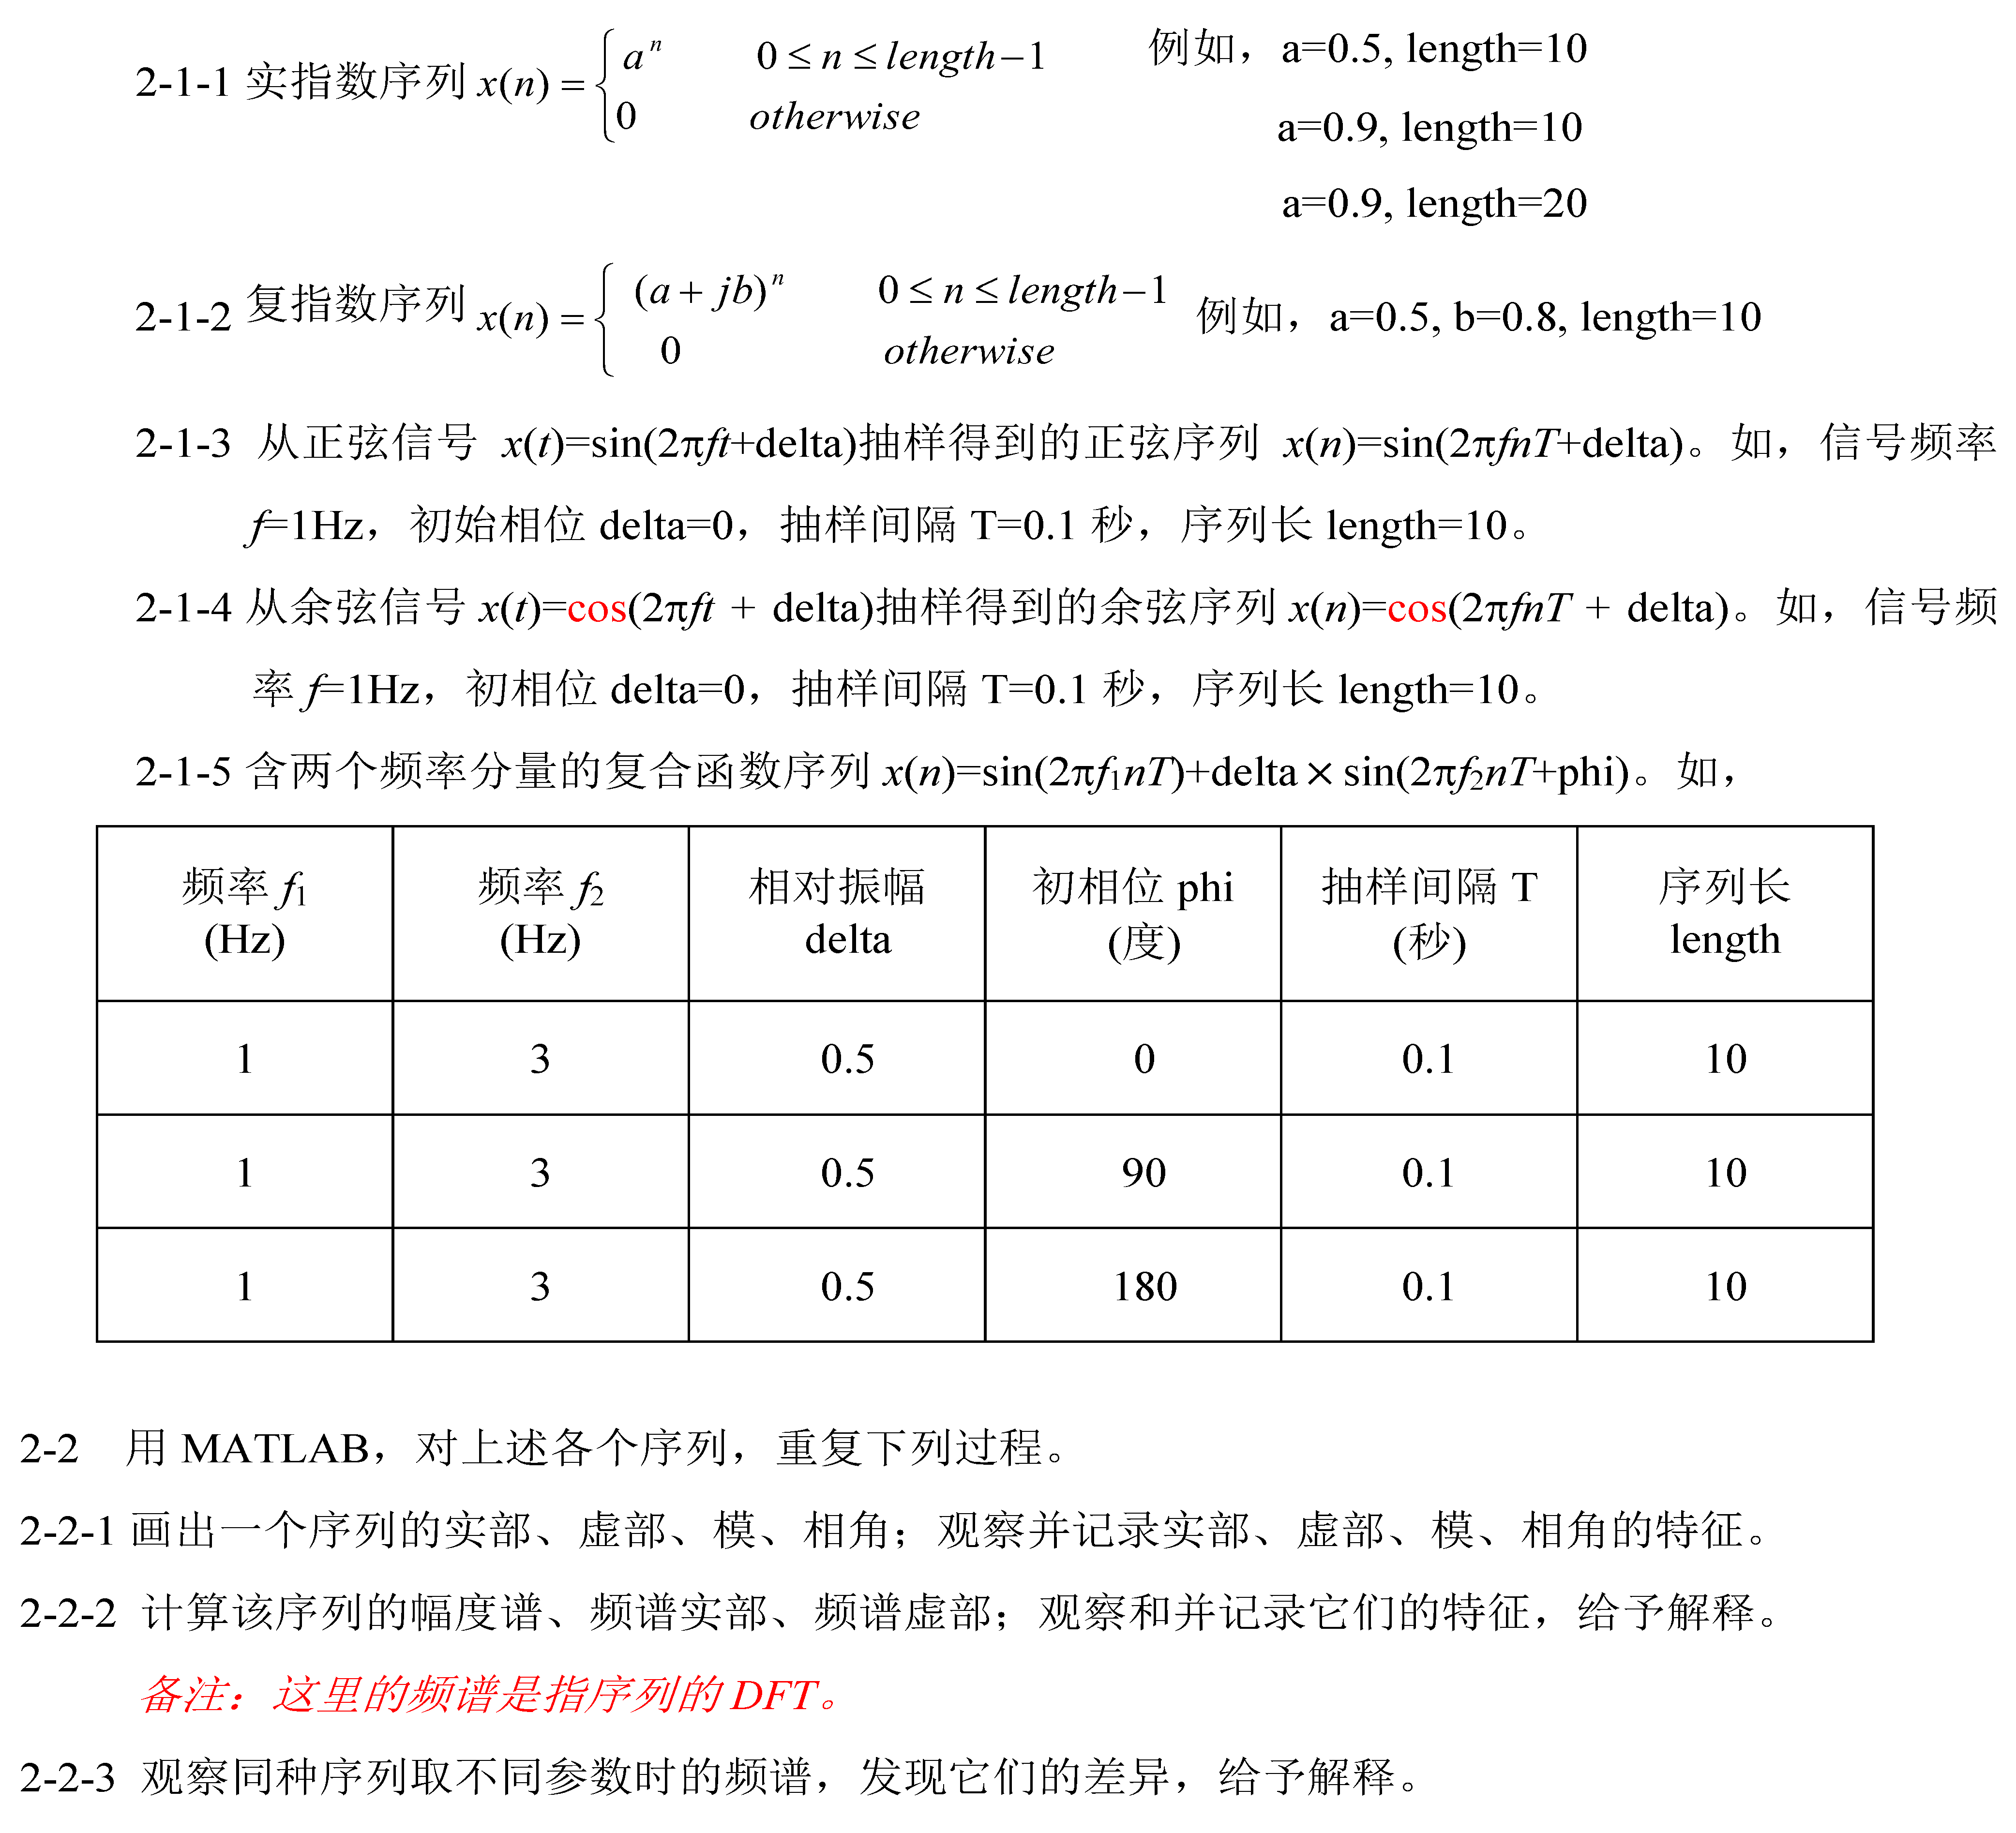
\includegraphics[width = 0.90\textwidth]{pic/2.png}
    \end{figure}
    \newpage

    \section{主要仪器设备}
    
    MATLAB编程。

    \section{操作方法和实验步骤}

    (参见“二、实验内容和步骤”)

    \section{实验数据记录和处理}

    \section{实验结果与分析}

\end{document}